%
% Template for Doctoral Theses at Uppsala
% University. The template is based on
% the layout and typography used for
% dissertations in the Acta Universitatis
% Upsaliensis series
% Ver 5.2 - 2012-08-08
% Latest version available at:
%   http://ub.uu.se/thesistemplate
%
% Support: Wolmar Nyberg Akerstrom
% Thesis Production
% Uppsala University Library
% avhandling@ub.uu.se
%
%%%%%%%%%%%%%%%%%%%%%%%%%%%%%%%%%%%%%%%%%%%


%\documentclass{UUThesisTemplate}
\documentclass[11pt,a4paper,twoside,openany]{report}

\author{Albin Stjerna}
\date{\today}

% Package to determine wether XeTeX is used
\usepackage{ifxetex}

\ifxetex
	% XeTeX specific packages and settings
	% Language, diacritics and hyphenation
        \usepackage[babelshorthands]{polyglossia}
        \usepackage{xunicode}
	\setmainlanguage{english}
	%\setotherlanguages{swedish}

	% Font settings
	\setmainfont{Baskerville}
  \setromanfont{Baskerville}
	\setsansfont{Helvetica Neue}
	%\setmonofont{Source Code Pro} % only minted!
\else
	% Plain LaTeX specific packages and settings
	% Language, diacritics and hyphenation
    % Use English and Swedish languages.
	\usepackage[british]{babel}

	% Font settings
	\usepackage{type1cm}
	\usepackage[latin1]{inputenc}
	\usepackage[T1]{fontenc}
	\usepackage{mathptmx}

	% Enable scaling of images on import
	\usepackage{graphicx}
\fi

\usepackage{listings}
\usepackage{fancyvrb}
\usepackage{multicol}
\usepackage[font={small,it}]{caption}

% Tables
\usepackage{booktabs}
\usepackage{tabularx}
\usepackage{bm}
\usepackage{longtable}
\usepackage{lipsum}
\usepackage{sectsty}

\usepackage[lining]{sourcecodepro}
\allsectionsfont{\normalfont\sffamily\bfseries}

\clubpenalty 4000
\widowpenalty 4000

% Document links and bookmarks
\usepackage{url}
\usepackage[xetex, colorlinks=true,
            linkcolor=blue, citecolor=blue,
            urlcolor=blue,breaklinks]{hyperref}
\usepackage[
    backend=biber,
    natbib=true,
    style=ieee,
    sorting=none,
    backref=true]{biblatex}
\bibliography{bibliography.bib}

% Numbering of headings down to the subsection level
%\numberingdepth{subsection}

% Including headings down to the subsection level in contents
%\contentsdepth{subsection}

\setlength{\columnsep}{0.2cm}
\usepackage{pdfpages}
\usepackage{mathtools}
\usepackage{varioref}
\usepackage{nowidow}
%\usepackage{cleveref}
\usepackage[toc,page]{appendix}
\newcommand{\fixme}[1] {{\color{red}#1}}
\newcommand{\notmine}[0] {$^\dagger$}
\usepackage{microtype}
\usepackage[newfloat]{minted}
\usepackage{caption}

\newenvironment{sourcecode}{\captionsetup{type=listing}}{}
\SetupFloatingEnvironment{listing}{name=Listing}
\usepackage{csquotes}
\usemintedstyle{xcode}
\setminted{fontsize=\footnotesize}

\setnowidow[5]
\setnoclub[3]

\newcommand{\InRust}[1]{\mintinline{rust}{#1}}
\newcommand{\InDatalog}[1]{\mintinline{prolog}{#1}}

\newcommand{\RustBlock}[3]{
  \begin{sourcecode}
    \captionof{listing}{#2}
    \label{code:#1}
\begin{minted}{rust}
#3
\end{minted}
  \end{sourcecode}}

% Uncomment to use a custom abstract dummy text
%\abstractdummy{
% }

\usepackage{xparse}
%
\DeclarePairedDelimiterX{\Set}[1]{\{}{\}}{\setargs{#1}}
\NewDocumentCommand{\setargs}{>{\SplitArgument{1}{;}}m}
{\setargsaux#1}
\NewDocumentCommand{\setargsaux}{mm}
{\IfNoValueTF{#2}{#1} {#1\,\delimsize|\,\mathopen{}#2}}%{#1\:;\:#2}

\newcommand{\ntyperule}[2]{\begin{array}{c}#1\\\hline\raisebox{1pt}{\strut}#2\end{array}}

\title{Modelling Rust's Reference Ownership Analysis Declaratively in Datalog}

\begin{document}
% %\frontmatter*
%     % Creates the front matter (title page(s), abstract, list of papers)
%     % for either a Comprehensive Summary or a Monograph.
%     % Authors of Comprehensive Summaries use this front matter
%     %\frontmatterCS
%     % Monograph authors use this front matter
%     %\frontmatterMonograph

    % Environment used to create a list of papers
    % \begin{listofpapers}
    % 	\item A Paper Discussed in this Thesis \label{apaperlabel}
    % \end{listofpapers}

\maketitle

\section*{Abstract}
\textit{\fixme{This thesis is about something.}}


\begingroup
        % To adjust the indentation in your table of contents, uncomment and enter the widest numbers for each level
        %  E.g.  \settocnumwidth{widest chapter number}{widest section number}{widest subsection number}...{...}
       %  \settocnumwidth{5}{4}{5}{3}{3}{3}
  \tableofcontents
  %\listoffigures
  % \listoftables
\endgroup
  
%\section*{Acknowledgements}
%\fixme{I thank everyone for everything.}

\chapter{Introduction}
%\epigraph{\fixme{short quote}}
%\mainmatter{}
% what are the contributions made?
% why?

Rust is a young systems language originally developed at Mozilla
Research~\cite{matsakis_rust_2014}. Its stated intention is to combine
high-level programming language features like automatic memory management and
strong safety guarantees, in particular in the presence of concurrency or
parallellism, with predictable performance and pay-as-you-go abstractions in the
style of C++ and similar systems languages.

One of its core features is the memory ownership model, which enables
compile-time safety guarantees against data races, unsafe pointer dereferencing,
and runtime-free automatic memory management, including for dynamic memory
allocated on the heap.

This report describes the implementation of Rust's memory safety checker, called
the borrow checker, in an embedded Datalog engine, as well as its optimisation.
In practice, the full analysis encompasses a variable liveness analysis,
initialisation and deinitialisation tracking, and may-reference analysis for
validation of Rust's memory safety guarantees.

\fixme{mention results.}

\chapter{Background}
Whenever a reference to a resource is created in Rust, its borrowing rules
described in Section~\ref{sec:borrowing-rules} must be respected for as long as
the reference is alive, including across function
calls~\cite{nichols_rust_nodate}. In order to enforce these rules, the Rust
language treats the scope of a reference, called its lifetime, as part of its
type, and also provides facilities for the programmer to name and reason about
them as they would any other type.

% similar but different to Region-based memory

Since its release, the Rust compiler has been extended through proposal RFC~2094
to add support for so-called non-lexical lifetimes (NLLs), allowing the compiler
to calculate lifetimes of references based on the control-flow graph rather than
the lexical scopes of variables~\cite{noauthor_rfc_2019}. During the spring of
2018, Nicholas Matsakis began experimenting with a new formulation of the borrow
checker, called Polonius, using rules written in
Datalog~\cite{matsakis_alias-based_2018}. The intention was to use Datalog to
allow for a more advanced analysis while also allowing for better compile-time
performance through the advances done centrally to the fixpoint solving provided
by the Datalog engine used for the computations~\cite{datafrog}.

Datalog, and other types of logic programming has been previously employed for
program analysis, in particular pointer analyses such as may-point-to and
must-point-to analysis, both similar to what is described in this report in that
they require fix-point solving and graph traversal, often with a context
sensitive analysis (i.e. respecting function boundaries) like the
one described here\cite{Dawson:1996:PPA:231379.231399,
  Berndl:2003:PAU:780822.781144, hajiyev_codequest:_2005,
  Whaley:2004:CCP:996893.996859, lam_context-sensitive_2005,
  Benton:2007:ISD:1273920.1273923, Hardekopf:2007:AGF:1250734.1250767,
  Smaragdakis:2011:PYC:1926385.1926390, smaragdakis_using_2010,
  balatsouras_datalog_2017, Madsen:2016:DFD:2908080.2908096,
  Eichberg:2008:DCC:1368088.1368142}. These systems employ a wide variety of
solver technologies and storage back-ends for fact storage, from Binary
Decision Diagrams (BDDs) to explicit tuple storage, as used in this study. Some
of them, like \textsc{Flix}, also extends Datalog specifically for static
program analysis\cite{Madsen:2016:DFD:2908080.2908096}.

In addition to being context-sensitive, Rust's borrow checker is also
flow-sensitive (i.e. performs analysis for each program point), like the system
described by \citeauthor{Hardekopf:2009:SFP:1480881.1480911}, and whose form is
very similar to the analysis performed in practice by
Polonius~\cite{Hardekopf:2009:SFP:1480881.1480911}.

A \citeyear{scholz_fast_2016}~study uses the Souffl{\'e} system, which
synthesizes performant C++ code from the Datalog specifications, similar to how
Datafrog embeds a minimal solver as a Rust library, to show promising
performance for analysis of large programs~\cite{scholz_fast_2016}. The
\textsc{Doop} system, developed by \citeauthor{smaragdakis_using_2010}, also
shows that explicit tuple storage sometimes vastly outperforms BDDs in terms of
execution time~\cite{smaragdakis_using_2010}, as do sparse
bitmaps~\cite{Hardekopf:2007:AGF:1250734.1250767}.

Formally, the semantics of Rust's lifetime rules has been captured in the
language Oxide, described by
\citeauthor{weiss_oxide:_2019}~\cite{weiss_oxide:_2019}. This report will
therefore not concern itself with the semantics of the borrow rules, except
where necessary to explain the rules.

% UPDATE: make sure that this section is up to date:
The contributions made within the scope of the thesis project specifically
includes the implementation of liveness and initialisation calculations
(Sections~\ref{sec:var-livenes} and~\ref{sec:var-initalisation} respectively),
as well as work on region inference for higher-ranked types. Finally, the report
also evaluates the runtime performance of the system and suggests some potential
optimisations in Section~\ref{sec:optim-borr-check}, and performs a field study
of the shape of input data in Section~\ref{sec:field-study-borrow}. The core
rules of Polonius for the region constraints were already written when the
project started, but are described in Section~\ref{sec:fixme} for completeness.
For clarity, sections not developed by me are marked with daggers~(\notmine{}).

\section{The Borrowing Rules}\label{sec:borrowing-rules}
Most of these examples are borrowed from
\citeauthor{weiss_oxide:_2019}~\cite{weiss_oxide:_2019}.

\begin{description}  
\item[Variables must be provably initialised before use] Whenever a variable is
  used, the compiler must be able to tell that it is guaranteed to be
  initialised:
  \begin{minted}{rust}
     let x: u32;
     let y = x + 1; // ERROR: x is not initialised
  \end{minted}
\item[A move deinitialises a variable] Whenever ownership of a variable is
  passed on (\emph{moved} in Rust parlance), e.g. by a method call or
  reassignment, the variable becomes deinitialised:
  \begin{minted}{rust}
    struct Point(u32, u32);
    
    let mut pt = Point(6, 9);
    let x = pt;
    let y = pt; // ERROR: pt was already moved to x
  \end{minted}
\item[There can be any number of shared references] A shared reference, also
  called a \textit{borrow} of a variable, is created with the \InRust{&}
  operator, and there can be any number of simultaneously live shared references
  to a variable:
  \begin{minted}{rust}
    struct Point(u32, u32);
    
    let mut pt = Point(6, 9);
    let x = &pt;
    let y = &pt; // This is fine
  \end{minted}
\item[There can only be one simultaneous live unique reference] Whenever a
  unique reference is created, with \InRust{&mut}, it must be unique:
  \begin{minted}{rust}
    struct Point(u32, u32);
    
    let mut pt = Point(6, 9);
    let x = &mut pt;
    let y = &mut pt; // ERROR: pt is already borrowed
    
    // code that uses x and y
  \end{minted}

  This error happens even if the first borrow is shared, but not if
  either \InRust{x} or \InRust{y} are dead (not used).
  
\item[A reference must not outlive its referent] A reference must go out of
  scope at the very latest at the same time as its referent, which protects
  aganst use-after-frees:
  \begin{minted}{rust}
    struct Point(u32, u32);
    
    let x = {
        let mut pt = Point(6, 9);
        &pt
    };
    
    let z = x.0; // ERROR: pt does not live long enough
  \end{minted}

  In this example, we try to set \InRust{x} to point to the variable \InRust{pt}
  inside of a block that has gone out of scope before \InRust{x} does.
\end{description}


\section{The Borrow Check in the Rust Compiler}
\label{sec:rust-specificts}

The logic of the borrow check as described in
Section~\ref{sec:reference-provenance} is calculated at the level of an
intermediate representation of Rust called the Mid-Level Intermediate
Representation (MIR), corresponding to the basic blocks of program control flow.
The input data to the Polonius solver is generated in the Rust compiler by
analysing this intermediate representation. This means that we can safely assume
to be working with simple variable-value assignment expressions, of the type
\InRust{_1 = _2}.

% Removed because we never actually calculate these in the report
% \fixme{Rust uses \emph{supporting prefixes} to refer to the parts of a variable
%   access path touched by a dereferencing in the MIR~\cite{noauthor_rfc_2019}.
%   This becomes important when determining which parts of a reference to consider
%   under borrowing constraints. For example, given a tuple with a reference
%   \InRust{r: (&(i32, i64), (f32, f64))}, the path \InRust{(*r.0).1} has type
%   \InRust{i64} and the supporting prefixes \InRust{(*r.0).1} and \InRust{*r.0}
%   (\InRust{*} has a low precedence and so it \InRust{*r.0} is the same as
%   \InRust{*(r.0)}). Similarly, the path \InRust{r.1.0} has the supporting
%   prefixes \InRust{r.1.0}, \InRust{r.1}, and \InRust{r}}.

\section{From Lifetimes to Provenance Variables}
\label{sec:reference-provenance}

As the lifetime of its value is a part of a variable's type, it can be referred
to by name like any other type using the syntax \InRust{&'lifetime}. In the
literature, the terms ``region''~\cite{matsakis_alias-based_2018}, ``(named)
lifetime''~\nocite{noauthor_rfc_2019}, and ``reference
provenance''~\cite{weiss_oxide:_2019} (provenance) are all employed. As the
section heading suggests, I will use the last one of them as I believe it best
captures the concept. Named provenances (such as \InRust{'lifetime} above) are
referred to as ``provenance variables''.

From a type system perspective, the provenance is part of the type of any
reference and corresponds to the borrow expressions that might have generated it
in the Polonius formulation of the borrow check. For example, if a reference
\InRust{r} has the type \InRust{&'a Point}, \InRust{r} is only valid as long as
the terms of the loans in \InRust{'a} are upheld. Take for example the code of
Listing~\ref{lst:multi-path-borrow}, where \InRust{p} would have the type
\InRust{&'a i32} where \InRust{a} is the set $\Set{L_0, L_1}$.

\begin{sourcecode}
  \captionof{listing}{An example of a multi-path
    borrow.}\label{lst:multi-path-borrow}
\begin{minted}{rust}
let x = vec![1, 2];

let p: &'a i32 = if random() {
  &x[0] // Loan L0
} else {
  &x[1] // Loan L1
};
\end{minted}
\end{sourcecode}

If a reference is used in an assignment like \InRust{let p: &'b i32 = &'a x},
the reference, \InRust{p}, cannot outlive the assigned value, \InRust{x}. More
formally the type of the right-hand side, \InRust{&'a i32}, must be a subtype of
the left-hand side's type; \InRust{&'a i32 <: &'b i32}. In practice, this
establishes that \InRust{'b} lives at most as long as \InRust{'a}, which means
that the subtyping rules for regions establishes a set membership constraint
between the regions, as seen in Rule~\ref{eq:subtype}.

\begin{equation}\label{eq:subtype}
\ntyperule{a \subseteq b}{\InRust{&'a u32} <: \InRust{&'b u32}}
\end{equation}

\fixme{How to incorporate the fact that this is with respect to the current point?}

Finally, when talking about the \emph{liveness} of a provenance variable $r$, we
will mean that $r$ occurs (\fixme{what does occurs mean? Does it encompass
  exploded subset-types etc?}) in the type of at least one live variable at some
point in the control-flow graph $p$. This has the semantic implication that any
of the loans in $r$ might be dereferenced at control-flow points reachable from
$p$, and thus that the terms of the loans in $r$ must be respected at that
point.


\section{Deallocation As a Special Case of Variable Use}
\label{sec:deall-as-spec}
When Rust's variables go out of scope, they are implicitly deallocated, or
dropped in Rust parlance. Explicit deallocation is also possible by calling the
function \InRust{drop()}, which takes ownership of a variable and performs
deallocation, or, for complex objects, calls the \InRust{drop()} method. For
some types such as integers, deallocation is not necessary and the
compiler generates no actual \InRust{drop()}:s in the MIR.

Rust provides a default deallocator for data structures, but it can be
overridden. This has repercussions on liveness calculations, because while the
default deallocator for an object never needs to access its fields, a custom
deallocator might access any of them. This means that any conditions of a loan
that resulted in a reference $r$ stored in a \InRust{struct} $s$ instance $a$
must only be respected as far as \InRust{a.drop()} is concerned if $s$
implements a custom deallocator. Otherwise the loan of $r$ may be safely
violated, as the default deallocator never dereferences $r$ and thus doesn't
require $r$ to be valid. An illustration of this can be seen in
Listing~\ref{lst:drop-liveness}.

\begin{sourcecode}
  \captionof{listing}{The custom deallocator for \InRust{OwnDrop} enforces the
    loan of \InRust{data}, but the loan in \InRust{OwnDrop} is effectively dead
    and thus can be violated.}\label{lst:drop-liveness}
\begin{minted}{rust}
struct OwnDrop<'a> {
    data: &'a u32,
}

struct DefaultDrop<'a> {
    data: &'a u32,
}

impl<'a> Drop for OwnDrop<'a> {
    fn drop(&mut self) {
        // might access self.data
    }
}

fn main() {
    let mut x = 13;
    let a = OwnDrop { data: &x };

    let mut y = 12;
    let b = DefaultDrop { data: &y };
    
    // let mutrefa = &mut x;
    // ERROR: the loan of x must be respected...
    
    // ...but the loan of y need not be!
    let mutref = &mut y;
    *mutref = 17;
    
    // all variables are implicitly dropped here
}
\end{minted}
\end{sourcecode}

\section{Datalog and Datafrog}
\label{sec:datalog}

Datalog is a derivative of the logic programming language Prolog, with \fixme{x
  guarantees about execution}. It describes fixpoint calculations over logical
relations as predicates, described as fixed input \emph{facts}, computed
\emph{relations}, or \emph{rules} describing how to populate the relations based
on facts or other relations. For example, defining a fact describing that an
individual is another individual's parent might look like
\InDatalog{parent(mary, john).}, while computing the \InDatalog{ancestor}
relation could use the two rules \InDatalog{ancestor(X, Y) :- parent(X, Y).} and
\InDatalog{ancestor(X, Y) :- parent(X, Z), ancestor(Z, Y).}, reflecting the fact
that ancestry is respectively either parenthood or transitive parenthood
(example from the Wikipedia article on Datalog~\cite{wiki:datalog}). This thesis
uses the notation of Souffl{\'e}~\cite{scholz_fast_2016}.


Datafrog~\cite{datafrog} is a minimalist Datalog implementation embedded in
Rust, providing an implementation of a worst-case optimal join algorithm as
described in~\cite{ngo_worst-case_2012}. The fact that Datafrog is embedded in
Rust means that standard Rust language abstractions are used to describe the
computation. Static facts are described as \InRust{Relation}s, while
\InRust{Variable}s are used to capture the results of computations, both of
which are essentially sets of tuples. Rules are described using a join with
either a \InRust{Variable} or an \InRust{Relation}, with an optimised join
method for joins with the variable itself. Only single-step joins on the first
tuple element are possible, which means that more complex rules must be written
with intermediary variables, and manual indices created whenever a relation must
be joined on a variable which is not the first in the tuple.

\begin{sourcecode}
  \captionof{listing}{The implementation of \InDatalog{var_live(V, P)} in
    Datafrog.}\label{lst:datafrog:var-live}
\begin{minted}{rust}
var_live_var.from_leapjoin(
    &var_live_var,
    (
        var_defined_rel.extend_anti(|&(v, _q)| v),
        cfg_edge_reverse_rel.extend_with(|&(_v, q)| q),
    ),
    |&(v, _q), &p| (v, p),
);
\end{minted}
\end{sourcecode}


As an example, the Datafrog code for \InDatalog{var_live(V, P)} of
Listing~\ref{lst:var-live} becomes the code in
Listing~\ref{lst:datafrog:var-live}, and the corresponding join used for the
first half of \InDatalog{region_live_at(R, P)} of
Listing~\ref{lst:region-live-at} can be seen in
Listing~\ref{lst:datafrog:region-live-at}.

\begin{sourcecode}
  \captionof{listing}{The first half of the implementation of
    \InDatalog{region_live_at(R, P)} in
    Datafrog.}\label{lst:datafrog:region-live-at}
\begin{minted}{rust}
region_live_at_var.from_join(
    &var_drop_live_var, 
    &var_drops_region_rel, 
    |_v, &p, &r| {
        ((r, p), ())
    });
\end{minted}
\end{sourcecode}


\chapter{A Datalog Model for the Rust Borrow Checker}
\label{cha:investigation}
% \epigraph{\fixme{short quote}}


\section{The Borrow Checker in Datalog}

\subsection{Starting Facts}
\label{sec:input-facts}

The following short-hand names are used:
\begin{description}
\item[$R$] is a provenance.
\item[$L$] is a loan, that is an \InRust{&v} expression creating a reference
  to \InRust{v}.
\item[$P, Q$] are points in the control-flow graph of the function under analysis.
\item[$V$] is a variable.
\end{description}


\begin{description}
\item[\InDatalog{borrow_region(R, L, P)}] the provenance~$R$ may refer
  to data from loan $L$ starting at the point $P$ (this is usually the point
  \emph{after} the right-hand-side of a borrow expression).
  
\item[\InDatalog{universal_region(R)}] for each named/parametrised provenance
  variable~$R$ supplied to the function. $R$ is considered universally
  quantified, and therefore live in every point of the function.
  
\item[\InDatalog{cfg_edge(P, Q)}] whenever there is a relation $P \rightarrow Q$
  in the control flow graph.
    
\item[\InDatalog{killed(L ,P)}] when some prefix of the path (\fixme{explain
    prefixes and paths}) borrowed in $L$ is assigned at point~$P$.
    
\item[\InDatalog{outlives(R1, R2, P)}] when $R_1 \subseteq R_2$ must hold at
  point~$P$, a consequence of subtyping relationships as described in
  Rule~\eqref{eq:subtype}.
    
\item[\InDatalog{invalidates(P, L)}] when the loan~$L$ is invalidated by some
  operation at point~$P$.
    
\item[\InDatalog{var_used(V, P)}] when the variable~$V$ is used for anything but
  a drop at point~$P$.
    
\item[\InDatalog{var_defined(V, P)}] when the variable~$V$ is assigned to
  (killed) at point~$P$.
  
\item[\InDatalog{var_drop_used(V, P)}] when the variable~$V$ is used in a drop at point~$P$.

\item[\InDatalog{var_uses_region(V, R)}] when the type of~$V$ includes the
  provenance~$R$.

\item[\InDatalog{var_drops_region(V, R)}] when the type of~$V$ includes the
  provenance~$R$, and~$V$ also implements a custom drop method which might need
  all of~$V$'s data, as discussed in Section~\ref{sec:deall-as-spec}.
\end{description}


\subsection{Reference Liveness}
\label{sec:var-livenes}

The basic liveness of a variable (Listing~\ref{lst:var-live}) is defined as
follows: if a variable~$v$ is live in some point~$q$ and~$q$ is reachable from
$p$ in the control-flow graph, then~$v$ is live in~$p$ too unless it was
overwritten; in essence liveness is propagated backwards through the CFG.

\begin{sourcecode}
  \captionof{listing}{The Datalog rules for variable
    use-liveness.}\label{lst:var-live}
\begin{minted}{prolog}
var_live(V, P) :-
    var_live(V, Q),
    cfg_edge(P, Q),
    !var_defined(V, P).
\end{minted}
\end{sourcecode}


There is also a very similar relation for drop-liveness with an identical shape
and different input relations corresponding to drop-uses. An example of the
output from this calculation can be seen in Figure~\ref{fig:liveness-graph}.

Both of these are then used to calculate the reference liveness relation
(Listing~\ref{lst:region-live-at}), which serves as input for the rest of the
borrow checker. A given provenance~$r$ is live at some point~$p$ if it is in the
type of a variable~$v$ which is either drop-live or use-live at~$p$, with some
notable caveats for drop-liveness (discussed in Section~\ref{sec:deall-as-spec})
embedded in the \InDatalog{var_drops_region} relation.

\begin{sourcecode}
  \captionof{listing}{The Datalog rules for provenance
    liveness.}\label{lst:region-live-at}
\begin{minted}{prolog}
region_live_at(R, P) :-
    var_drop_live(V, P),
    var_drops_region(V, R).
        
region_live_at(R, P) :-
        var_live(V, P),
        var_uses_region(V, R).
\end{minted}
\end{sourcecode}

\begin{figure}
  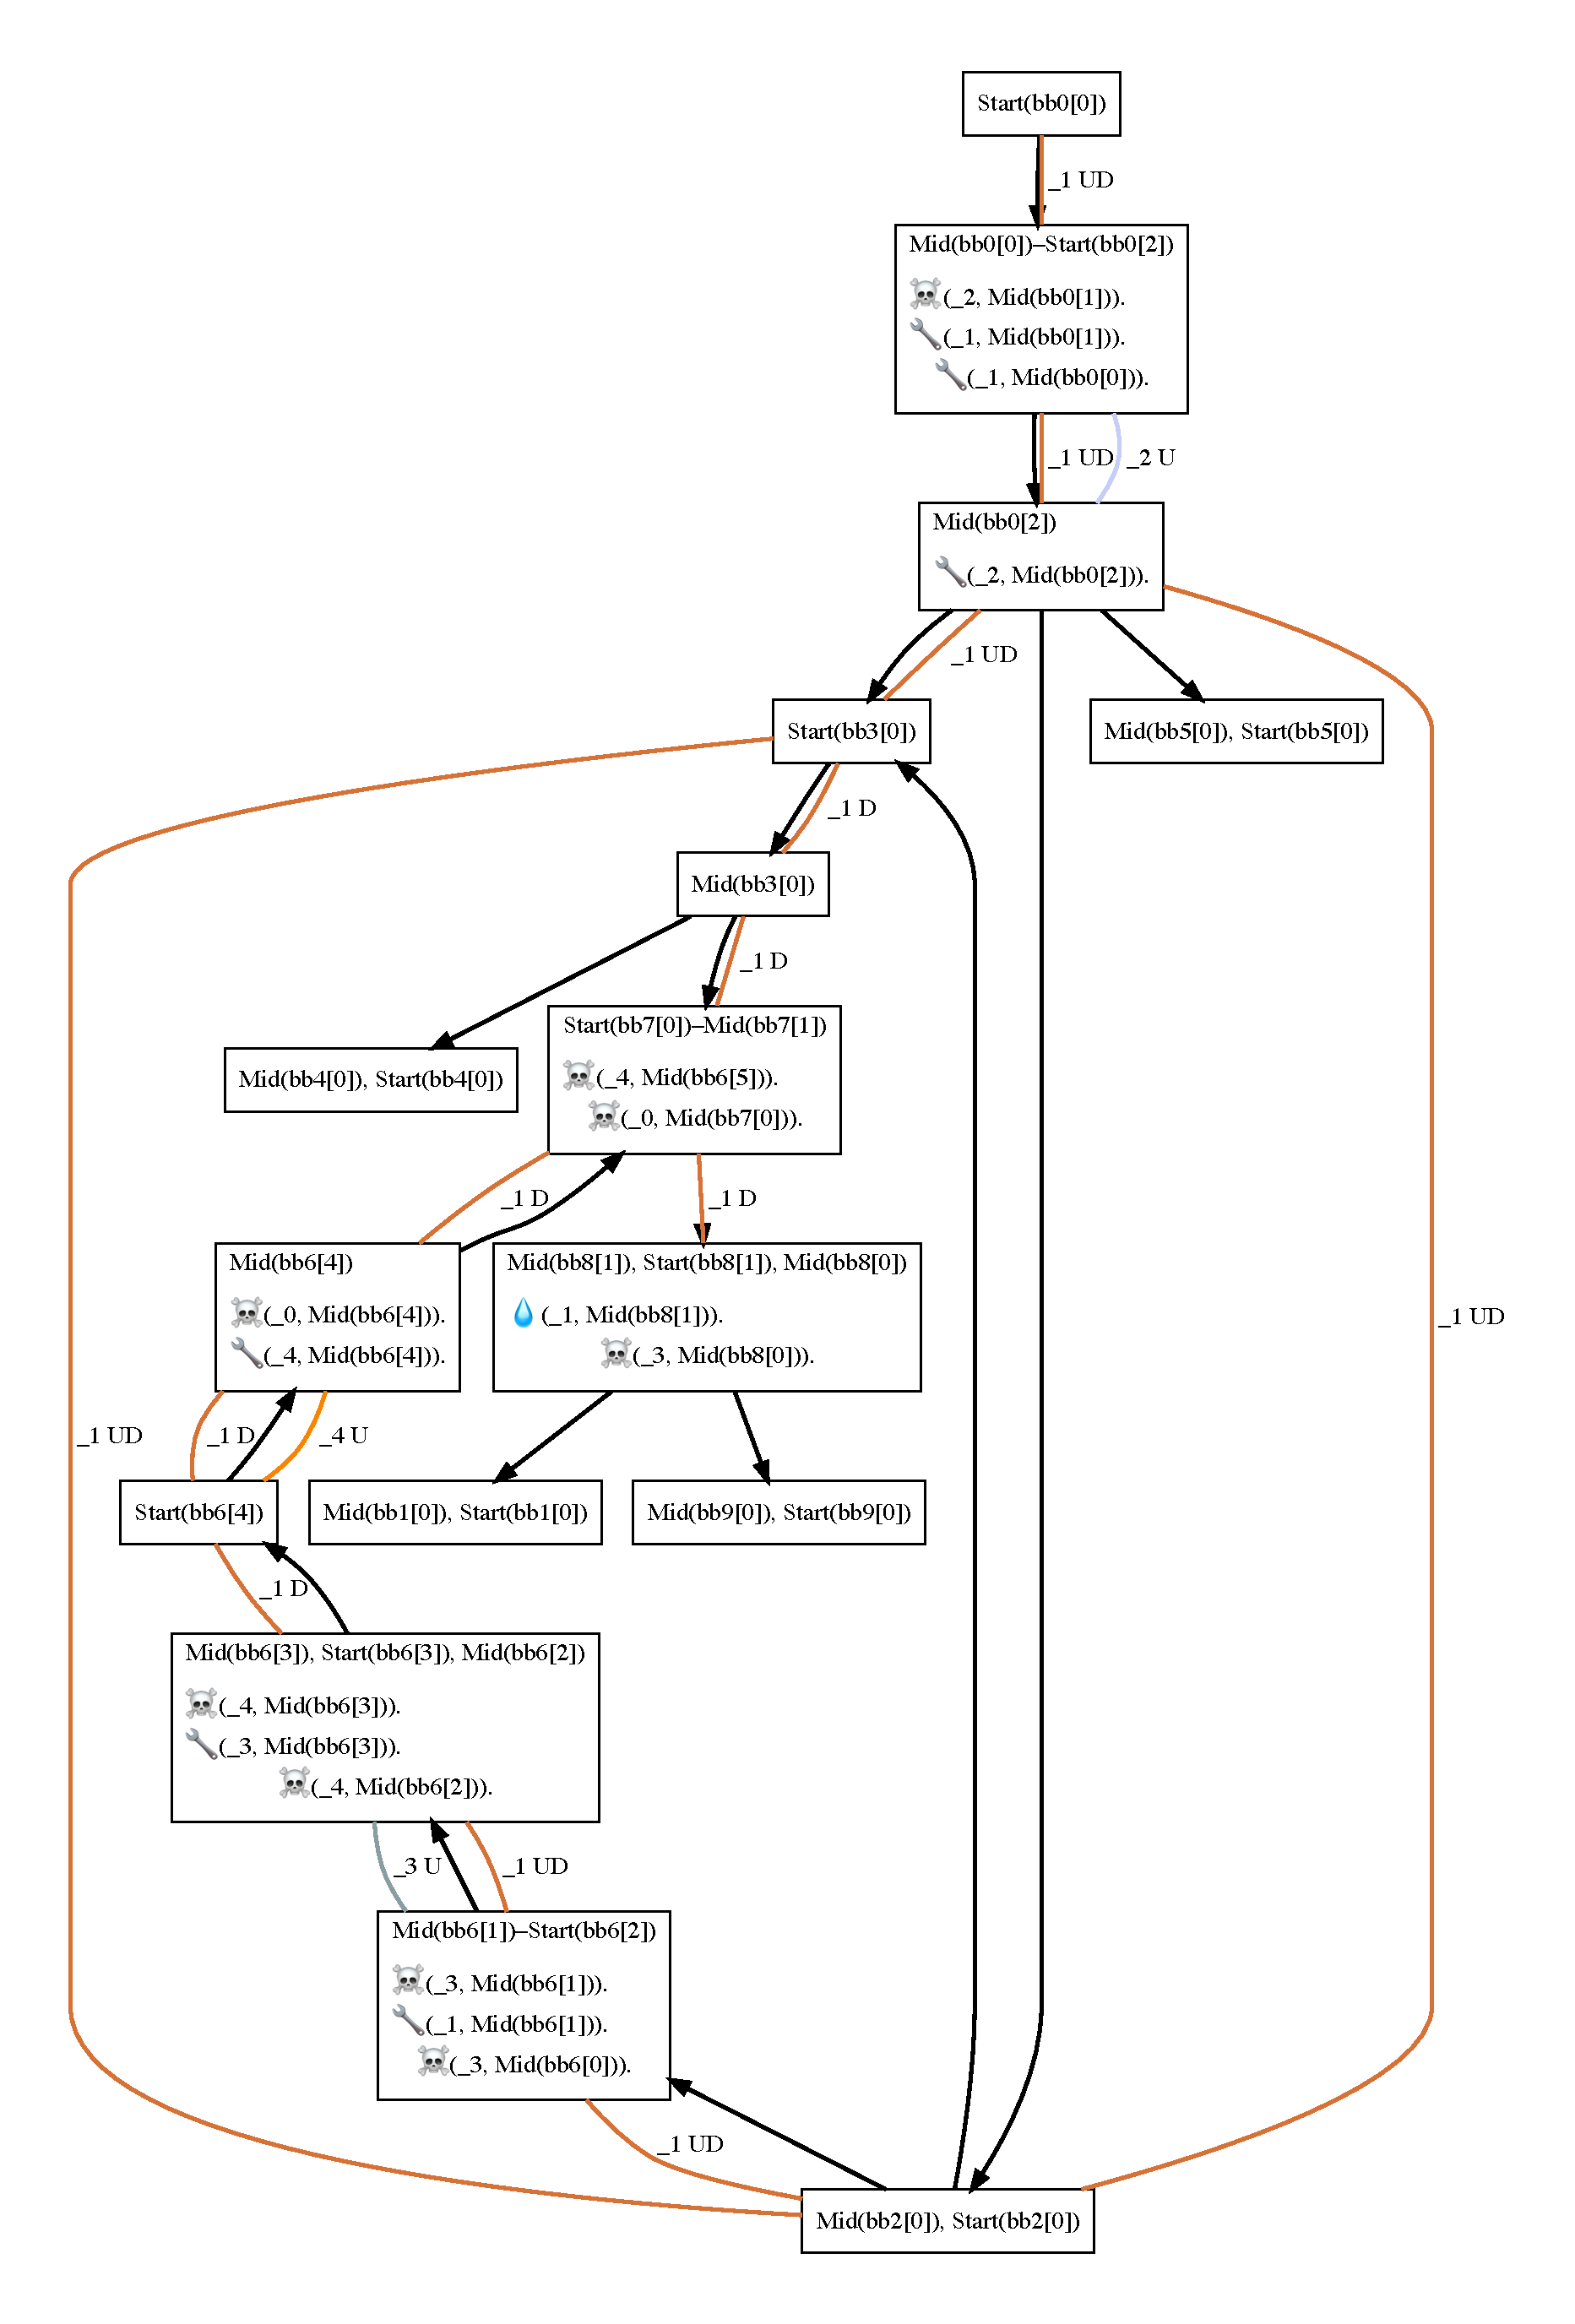
\includegraphics[width=0.9\linewidth]{Graphs/liveness.pdf}
  \caption{A graph representation of the the variable liveness calculation
    results, with relevant Polonius facts as they occur (a droplet symbolising
    \InDatalog{var_drop_used}, a wrench \InDatalog{var_used}, and a skull and
    crossbones symbolising \InDatalog{var_defined}). Variables are named by
    prefixing underscores, and edges annotated with the propagated live variable
    and its liveness type(s) (\textbf{D}rop or \textbf{U}se).}
  \label{fig:liveness-graph}
\end{figure}

\subsection{Variable Initialisation}
\label{sec:var-initalisation}


\subsection{Loan Constraint Propagation\notmine{}}

\subsection{Loan Violations\notmine{}}

\subsection{Illegal Subset Relations\notmine{}}

\section{A Field Study of Borrow Patterns}\label{sec:field-study-borrow}

\section{Optimising the Borrow Checker}\label{sec:optim-borr-check}

% implied constraints, symmetries, optimisations

\chapter{Conclusions and Future Work}\label{cha:conclusions}
%\epigraph{\fixme{short quote}}

%\begin{appendices}
%\end{appendices}

%\backmatter
\printbibliography[heading=bibintoc]
\end{document}
